\clearpage
\section{Come riportare problemi e anomalie}
	\begin{enumerate}
		
		\item La segnalazione di problemi e malfunzionamenti avviene creando una \glossario{issue} di \glossario{GitHub} tramite il pulsante \emph{Report a problem} collocato nel \glossario{footer} di ogni pagina (Figura \ref{fig:probelmReportButton}).

		\begin{figure}[H]
				\label{fig:showpage}
					\centering 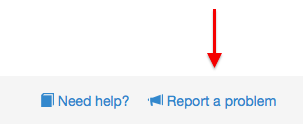
\includegraphics[width=0.6\textwidth]{img/probelmReportButton.png}
				\caption{\label{fig:probelmReportButton} Pulsante segnalazione anomalia}
		\end{figure}

		\item La pagina di report (Figura \ref{fig:paginaProbelmReport}) mostra un pulsante che permette di aprire una issue su \glossario{GitHub}, per eseguire tale operazione è necessario possedere un account di \glossario{GitHub}. Per aprire un account su \glossario{GitHub} andare su \url{https://github.com/join}, la procedura è guidata ben descritta nella pagina stessa.

		\begin{figure}[H]
				\label{fig:showpage}
					\centering 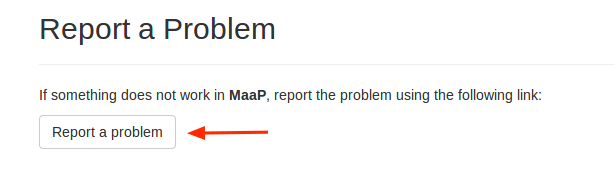
\includegraphics[width=1\textwidth]{img/paginaProbelmReport.png}
				\caption{\label{fig:paginaProbelmReport} Pagina segnalazione anomalia}
		\end{figure}

		\item La descrizione del problema dovrà contenere i seguenti punti:

		\begin{enumerate}
			\item Titolo della \glossario{issue} dovrà essere conciso e descrittivo del problema riscontrato. 
			\item Descrizione estesa delle operazioni che hanno portato all'anomalia, corredata di tutte le note ritenute utili alla comprensione del problema.
			\item Riferimento temporale;
			\item Azioni e pagine in cui si è riscontrato il problema;
			\item Codice dell'errore se visualizzato;
			\item Label di \glossario{GitHub} impostata su \emph{bug}.
		\end{enumerate}

	\end{enumerate}